\documentclass[dvipdfmx]{beamer}
%\usepackage{indentfirst}
\usepackage{pxjahyper}
\setlength{\parindent}{11pt}
% theme
\usefonttheme{professionalfonts}
\usetheme{Madrid}
\usecolortheme{default}
\setbeamertemplate{enumerate item}[default]
\setbeamertemplate{caption}[numbered]
\setbeamertemplate{navigation symbols}{}
\usepackage[scaled]{helvet}
\renewcommand{\sfdefault}{phv}
\renewcommand{\familydefault}{\sfdefault}
\renewcommand{\kanjifamilydefault}{\gtdefault}
\setbeamertemplate{theorems}[numbered]
\definecolor{Crimson}{HTML}{dc143c}
\setbeamercolor{alerted text}{fg=Crimson}
% graphics
\usepackage{graphicx}
\usepackage{here}

% math
\usepackage{amsmath, amssymb}
\usepackage{physics}
\usepackage{mathrsfs}
\usepackage{mathtools}
\usepackage[all]{xy}
\mathversion{bold}
\definecolor{math}{HTML}{100080}
\everymath{\color{math}}

% thorem
\usepackage{amsthm}
\newtheoremstyle{break}
{\topsep}{\topsep}%
{}{}%
{\bfseries}{}%
{\newline}{}%
\theoremstyle{break}
\newtheorem{thm}{Theorem}
\newtheorem{result}[thm]{SGEの結果}

% link

\usepackage{url}
\usepackage{hyperref} 
\usepackage{xcolor}
\usepackage{pxjahyper}
\definecolor{link}{HTML}{4b0082}
\hypersetup{
	colorlinks=true,
	citecolor=link,
	linkcolor=link,
	urlcolor=orange,
}

% my command
\newcommand{\up}{\ket{\uparrow}}
\newcommand{\down}{\ket{\downarrow}}
\newcommand{\C}{\mathbb{C}}
\newcommand{\R}{\mathbb{R}}
\renewcommand{\thefootnote}{\roman{footnote}}
% title
\author[@tos\_shiii]{}
\institute[Twitter]{}
\title[\textcolor{white}{SGEから始めるQM}]{数物系サーバー新歓ミニセミナー\\
Stern--Gerlachの実験から始める量子力学}

\begin{document}
\begin{frame}
		\maketitle
\end{frame}


\begin{frame}{はじめに}
		まず,聴衆のみなさんのバックグラウンドをお尋ねします.

		\begin{enumerate}
				\setbeamertemplate{items}[default]
				\item 新B1の方.\label{num:b1}
				\item 量子力学なんてなにもわからないよ,という方.\label{num:intro}
				\item ちょっとだけ勉強したことがあるよ,という方.
				\item 量子力学を完全に理解していて,冷やかしに来た方.
		\end{enumerate}

		\ref{num:b1}, \ref{num:intro}あたりの方に向けた雑談程度の講演であることはご理解ください.
\end{frame}


\begin{frame}{Introduction}
		量子力学の教科書の最初の話題は,古典論が破綻する実験事実が書かれることが多い.
		\begin{block}{伝統的なIntroduction}
		\begin{itemize}
				\item 黒体輻射\cite[\S1.1]{BN10398292}
				\item 光電効果\cite[\S1.2]{BN10398292}
				\item Compton散乱\cite[\S1.3]{BN10398292}, \cite[\S1.1, (1)]{BN0611143X}
				\item Bohrの原子模型\cite[\S1.6]{BN10398292}, \cite[\S1.1, (2)]{BN0611143X}
		\end{itemize}
		歴史的には重要であるが,破綻する古典論は統計力学・相対論など量子力学を習う段階ではしらないのが普通.
		\end{block}
		\begin{alertblock}{今回のIntroduction}
				\begin{itemize}
				\item Stern--Gerlachの実験 \cite{BC01962771}, \cite{BC08412531}
				\item 破綻する古典論は電磁気学
				\end{itemize}
		\end{alertblock}
\end{frame}


\begin{frame}{必要な古典論}
		本講演では,古典ではだめで量子論が必要であるということを感覚的に
		理解することが目的である.

		そのために必要な古典論の感覚を共有したい.

		\begin{columns}
				\begin{column}{0.7\textwidth}
						\begin{itemize}
								\item 電流は電子の流れであると考える.
								\item 電流のループがあると磁気モーメント$\vec{\mu}$が発生する.棒磁石みたいなイメージ.
								\item これを不均一磁場
%\footnote{不均一なのは,力を受けるようにするため.均一なら,偶力になって「回転」するだけだが,上下に強い磁石と弱い磁石を入れておくと強い方に力を受けて磁気モーメントの向きにより異なる力を受ける.}
										$\vec{B}$中に入れると,力$\vec{\nabla}(\vec{\mu}\cdot\vec{B})$を受ける.
								\item とにかく,\alert{力を受ける}こと,それが\alert{内積}で与えられることが大事.
								\item 内積なので,$\vec{\mu}$と$\vec{B}$のなす角$\theta\in[0, 2\pi)$による.
						\end{itemize}
				\end{column}
				\begin{column}{0.3\textwidth}
						\begin{figure}
								\centering
								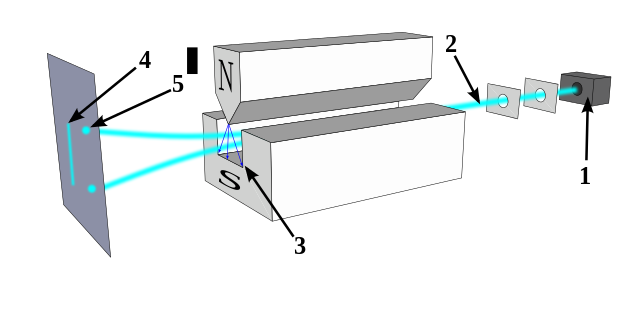
\includegraphics[scale=0.13, keepaspectratio]{./img/sg.png}
						\end{figure}
				\end{column}
		\end{columns}
\end{frame}


\begin{frame}[allowframebreaks]{SGの実験}
		\begin{columns}
		\begin{column}{0.6\textwidth}
		\begin{figure}[t]
				\centering
				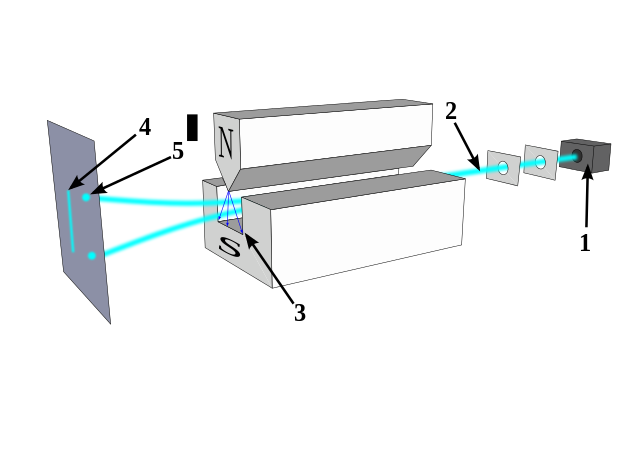
\includegraphics[keepaspectratio, scale=0.25]{./img/device.png}
				\caption{SGの実験装置.\href{https://en.wikipedia.org/wiki/Stern\%E2\%80\%93Gerlach_experiment}{Wikipedia}より拝借.}
		\end{figure}
		\end{column}
		\begin{column}{0.4\textwidth}
		\begin{enumerate}[SG1]
				\setbeamertemplate{items}[default]
				\item 電子発射装置
				\item 電子線
				\item 磁場\label{sge_dev}
				\item 古典論からの予測\label{sge_cl}
				\item 実験結果\label{sge_qm}
		\end{enumerate}
		\end{column}
		\end{columns}
		\begin{result}\label{sgx}
				\begin{itemize}
						\item 前述した古典論からは,角度$\theta$に応じて連続的に分布する.(SG\ref{sge_cl})
						\item 実際は\alert{上下二点のみ}に\alert{等しい強度}で現れる.(SG\ref{sge_qm})
				\end{itemize}
		\end{result}
		連続と思われていたものが実は離散だった,というのは他の導入にも共通している.

		この電子は二種類に分類できて,上の点にゆくものを$\up$,下の点にゆくものを$\down$と書くことにする.


		\begin{result}
				同じ設定で装置(SG\ref{sge_dev})を90度傾け,x方向の測定,y方向の測定,また,どれでもない斜めの方向の測定を行う.
				
				このとき,結果\ref{sgx}と同様に測定した方向に二点に分かれる.
		\end{result}
		\begin{result}
				装置を二つ用意して,z方向の測定を行った後$\up$だったものに対して,再びz方向の測定を行うと,$\up$しか観測できない.$\down$に関しても同様.
		\end{result}
		\begin{result}
				装置を二つ用意して,z方向の測定を行った後$\up$だったものに対して,x方向の測定をおこなうことを考える.
				このとき,電子はx方向に二点に分かれる.これに名前をつけて,$\ket{\rightarrow}$, $\ket{\leftarrow}$と呼ぶことにする.

				$\down$, y方向に関しても同様.
		\end{result}
		x方向の測定とz方向の測定は関係しないことがわかる.

		\begin{result}
				装置を三つ用意して,z方向の測定を行った後$\up$だったものに対して,x方向の測定を行う.この測定で$\ket{\rightarrow}$だったものに対して再びz方向の測定を行うと電子は二点に分かれる.

		\end{result}
%		\begin{align*}
%				\xymatrix@R=-10pt{
%						& & \up\\
%						&\ket{\rightarrow}\ar[ru]\ar[rd] & \\
%						& & \down\\
%						\up\ar[rdd]\ar[ruu] & & \\
%						& & \up\\
%						&\ket{\leftarrow}\ar[ru]\ar[rd] & \\
%						& & \down
%				}
%		\end{align*}
\end{frame}


\begin{frame}[allowframebreaks]{定式化}
		さて,以上のことは量子力学では次のように定式化される.

		\begin{block}{量子力学の定式化の一部}
				\begin{itemize}
						\item 電子の状態$\ket{\psi}$は$\up$, $\down$の線形結合でかける.すなわち$\ket{\psi}=c\up + d\down$, $c, d\in \C$.(重ね合わせ)
						\item $\up$, $\down$は次の意味で直交する.$\braket{\uparrow}{\downarrow} = \braket{\downarrow}{\uparrow} = 0$.規格化もしておく.$\braket{\uparrow}{\uparrow} = \braket{\downarrow}{\downarrow} = 1$.ここで$\braket{\bullet}{\bullet}$は内積である.
						\item 状態$\ket{\psi}$の電子にz方向の測定をしたとき,状態$\up$は確率$\abs{\braket{\uparrow}{\psi}}^2=\abs{c}^2$で観測される.$\down$についても同様.(確率解釈)
						\item $\up$を観測した場合,測定後の状態は$\up$になる.$\down$を観測した場合,$\down$になる.
				\end{itemize}
		\end{block}
		\newpage
		これを用いるとSGの実験結果は次のように説明できる.

		\begin{itemize}
				\item 一度目のz方向の測定では,$\up$, $\down$も完全にランダムにあると思うと,出現確率は$1/2$.
				\item 以降,一度目の測定で$\up$を観測したとする.
				\item 二度目にz方向の測定をすると,$\up$を観測する確率は$\abs{\braket{\uparrow}{\uparrow}}^2 = 1$, $\down$を観測する確率は$\abs{\braket{\uparrow}{\downarrow}}^2 = 0$.
				\item 二度目にx方向の測定を行うと,確率$1/2$で$\ket{\rightarrow}$, 確率$1/2$で$\ket{\leftarrow}$を観測した.これより
						\begin{align*}
								\ket{\rightarrow} = \frac{1}{\sqrt{2}}\up + \frac{1}{\sqrt{2}}\down,\quad
								\ket{\leftarrow} = \frac{1}{\sqrt{2}}\up - \frac{1}{\sqrt{2}}\down
						\end{align*}
						と構成できる.実際,先に述べたルールに従うと$\ket{\rightarrow}$が観測される確率は$\abs{\braket{\rightarrow}{\uparrow}}^2 = 1/2$である.
				\item 二度目に$\ket{\rightarrow}$だったとすると,測定後は$\ket{\rightarrow}$である.これより,三度目にz方向の測定を行うと,$\up$, $\down$がそれぞれ$1/2$の確率で出現する.
		\end{itemize}
\end{frame}


\begin{frame}{Summary}
		\begin{itemize}
				\item SGの実験は古典論では連続と思われるものが,離散的に分布することを見た.
				\item さらに,方向を変えたSGの実験を連続で行うと「不思議なこと」が起こった.

				\item これを量子力学の枠組みでどのように説明しているのかを述べ,具体的に計算した.

				\item 線形代数を習うと,この枠組みは二次元の計量付き線形空間論であることがわかる.
				\item 物理では,量子力学がその舞台であるミクロな素粒子などでもあらわれるのはもちろん,統計力学や低温のマクロなものにも本質的役割を果たす.
				\item 一般の量子力学は無限次元で議論されるので,数学の人はこれがHilbert空間やそのうえの作用素論になる.(勉強して教えて〜.)
				\item 以降の発展を示唆して,講演を終える.どうもありがとうございました.
		\end{itemize}
\end{frame}

\begin{frame}[allowframebreaks]{参考文献}
		\beamertemplatetextbibitems
		\bibliography{booklist}
		\bibliographystyle{jalpha}
\end{frame}
\end{document}

